\section{Budget} % income and outlays
The budget for the first year of the open data lab has a scope consisting of a purchase order for AWS time and personnel detailed from the Data Science Institute.

\begin{center}
Table of Income and Outlays for 2018

\begin{tabular}{lccr}
\hline
\hline
Source & Time (FTE) & Time (hours) & USD \\
\hline
\multicolumn{4}{c}{Income} \\
\hline
DSI Funds & && 6,000 \\
HM Funds & && 475 \\
Data Scientist & 1/2 & & \\
Clark Lab Dev & & 80 & \\
DSI Staff & & 100 & \\
\hline
Total Income & 1/2 FTE & 180 & 6,475 \\
\hline
\hline
\multicolumn{4}{c}{Outlays} \\
\hline
AWS & && 897 \\
Personnel Assigned & 1/2 FTE &  & \\
Personnel Temporary & & 180 & \\
\hline
Total Outlays & 1/2 FTE & 180 & 897 \\
\hline
\hline
Net & 0 & 0 & 5578 \\
\hline
\hline
\end{tabular}
\end{center}

\subsection{Income}
\begin{itemize}
\item Cash: The DSI allocated \$6,000 for computation and storage from AWS from the period of April 1, 2018 - March 31, 2019. These funds are drawn from PTAO 147242.102.LC00112.30002.
\item Cash: The Healthy Markets research project used ODL services for computation and storage on AWS. The ODL is authorized to transfer cost in proportion to the Healthy Markets PTAO 147412.107.DR03397.30002.
\item Personnel: The DSI allocated 50\% of a staff Data Scientist's time to the ODL project (1/2 FTE). The Clark lab contributed 80 hours of software developer time.
\end{itemize}
\subsection{Outlays}
\begin{itemize}
\item Cash: During 2018 the ODL spent \$897 on AWS.
\item Personnel: The ODL used the 1/2 FTE from the staff Data Scientist as well as a small ammount of time in meetings from various collaborators. AWS code development was contributed by Tim Clark's lab software developer.
\end{itemize}

\section{Balance Sheet} % assets and liabilities
At this time the Open Data Lab does not have any physical assets. There are digital assets including the materials stored on the github repository.

At this time the Open Data lab does not have any physical liabilities. There are liabilities in the form of commitments to ongoing research and education efforts in and around the DSI. Any decrease in support of personnel or funding will undermine the Open Data Lab's ability to cover those liabilities.

\begin{center}
Table of Assets and Liabilities for 2018

\begin{tabular}{lccr}
\hline
\hline
Source & Time (FTE) & Time (hours) & USD \\
\hline
\multicolumn{4}{c}{Assets} \\
\hline
\hline
Total Assets &  &  &  \\
\hline
\hline
\multicolumn{4}{c}{Liabilities} \\
\hline
AWS operations & 0.1\,FTE & &  \\
HM support & 0.1\,FTE &  & \\
DSI Capstone support & 0.1\,FTE & & \\
DSI Student support & 0.1\,FTE & & \\
DSI Research support & 0.1\,FTE & & \\
\hline
Total Liabilities & 1/2 FTE &  &  \\
\hline
\hline
Net & balance &  &  \\
\hline
\hline
\end{tabular}
\end{center}

Note further R\&D efforts are not included and require additional personnel. Also moving operations from beta to production requires additional FTE assignment and personnel would have to be hired to meet that need.

\subsection{FTE analysis}
Development progress was made before the start of the fall semester in August of 2018. However the role of the only FTE person on the ODL shifted to become a support role for the research and teaching mission of the DSI. From this three things are clear. 
\begin{enumerate}
\item There is a need for proficient computer support personnel for the DSI.
\item There is a need for proficient educational support personnel for the DSI.
\item If a ODLDS provides those services they will take more than 1/2 FTE.
\end{enumerate}
As a result for 2018 the development progress on the ODL came to a halt. Now we have a good estimate on the needs for support for the DSI, it is one FTE. If the DSI grows that number would increase. We recommend reaching out to Bryan Wright to serve on the hiring committee for this position.

Additionally the ODL never achieved a bus factor greater than 1 for any component. As a result there were substantial wait times and often service was delayed due to the FTE being already allocated.

\section{AWS usage}
To demonstrate the AWS usage we have extended the analysis window into 2019. 

The main driver of AWS cost is the usage of compute resources by research groups (see~\ref{fg:awstotal}. This was a surprising finding. Our belief was the data storage would be the driver. However only one project involved a data set greater than 1\,TB.
There were 22 S3 buckets created and six contain more than 10\,GB. Two buckets contain more data than is readily available on a laptop. Those are the wikipedia capstone bucket at 400\,GB. And the healthy markets bucket with 13.3\,TB.

The main driver of the compute cost was the use of ml.p2.xlarge instances through sagemaker. Those instances cost \$1.26/hour at time of writing. They are Tesla K80 GPUs from Nvidia with 61\,GB of conventional memory and 12\,GB of GPU memory.


\begin{figure}[!hbtp]
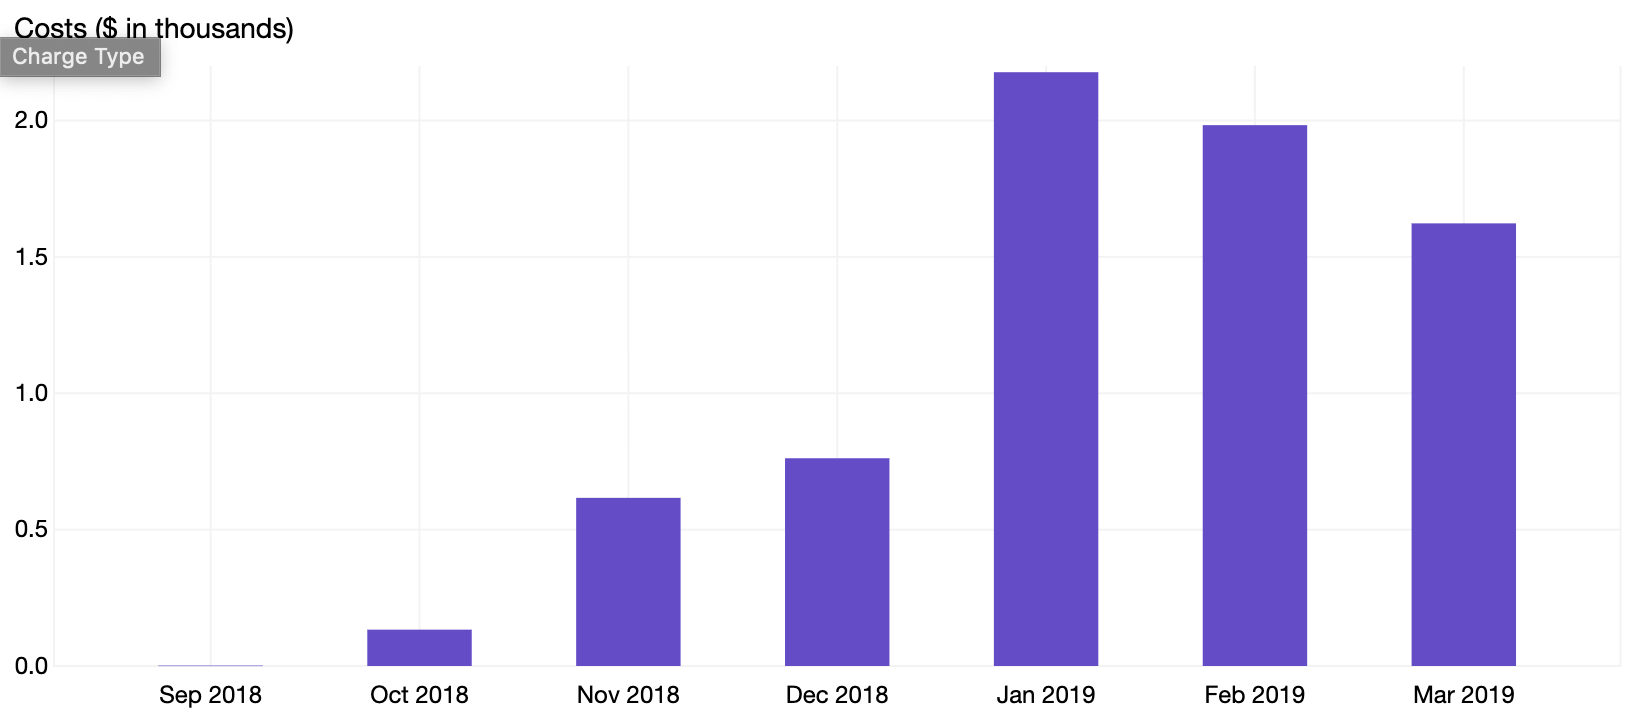
\includegraphics[width=\textwidth]{images/aws-metrics/throughmar/total.png}
\caption{AWS Total Costs\label{fg:awstotal}}
\end{figure}
\begin{figure}[!hbtp]
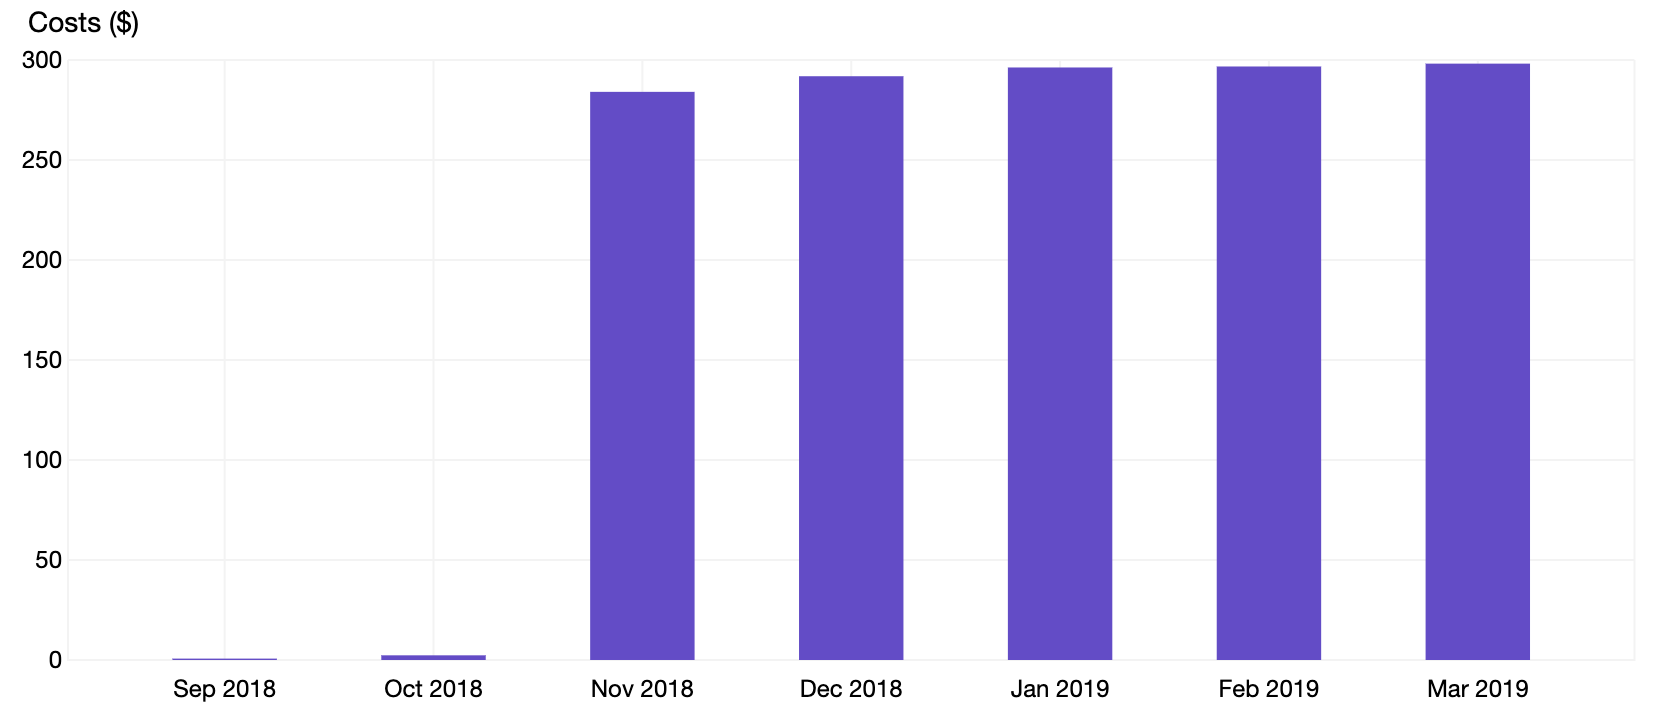
\includegraphics[width=\textwidth]{images/aws-metrics/throughmar/s3.png}
\caption{AWS S3 monthly costs. The main driver is 13.3\,TB for the Healthy Markets project\label{fg:awss3}}
\end{figure}


\section{Local UVA HPC usage}

\section{Funding Sources}
The ODL is funded by the DSI. The support for the Healthy Markets project is fronted by the ODL and then  cost transferred from the ODL PTAO to the HM PTAO.

